\documentclass[conference]{IEEEtran}
\IEEEoverridecommandlockouts
% The preceding line is only needed to identify funding in the first footnote. If that is unneeded, please comment it out.
\usepackage{cite}
\usepackage{amsmath,amssymb,amsfonts}
\usepackage{algorithmic}
\usepackage{graphicx}
\usepackage{textcomp}
\usepackage{xcolor}
\usepackage{algorithm2e}
\usepackage{amsmath}
\usepackage{tikz}
\usetikzlibrary{calc}
\usetikzlibrary{decorations.pathmorphing}
\usepackage{pgfplots}
\usepackage{float}

\graphicspath{ {./img/} }

\begin{document}

\title{CCTV Video Summarisation}

\author{\IEEEauthorblockN{
    AS Karthik\IEEEauthorrefmark{1},
    Abhishek Krishna\IEEEauthorrefmark{2},
    Gagan Deep G\IEEEauthorrefmark{3}
    and Dr. Ramakanth Kumar P\IEEEauthorrefmark{4}
}
\IEEEauthorblockA{Department of Computer Science,
RVCE\\
Bangalore\\
Email: \{\IEEEauthorrefmark{1}askarthik.cs15,
\IEEEauthorrefmark{2}abhishekkrishna.cs15,
\IEEEauthorrefmark{3}gagandeepg.cs15,
\IEEEauthorrefmark{3}ramakanthkumarp,
\}@rvce.edu.in
}}
\maketitle

\begin{abstract}
The use of CCTVs has been on the steady rise in in the last decade, being used for the security of public and private establishments alike. With increasing crime rates in cities, there is a need for a smarter method to survey the video being recorded, rather than manually going through hours of footage, saving both time and labour. We propose an efficient method to generate a summary of the footage. The project also aims to simplify the task further, by generating video summaries based on user query, thus showing exactly what is required.

\end{abstract}

\begin{IEEEkeywords}
CCTV, video summary, computer vision
\end{IEEEkeywords}

\section{Introduction}
\par
The number of CCTVs surveillance cameras is increasing everyday leading to
a huge amount digital video information being captured and stored. Millions of
CCTV cameras run 24 hours a day, sometimes even streaming the content over the
internet for people to monitor. This data is however in a raw, unprocessed
format.  In most cases, video with little to no motion is being captured,
which wastes lot of storage. The process of watching or analysing the footage is
also time consuming and laborious.

This project proposes to build a CCTV video summariser to eliminate this
redundancy in stored data and give the user a short summary\cite{oh2005video}, \cite{nam1999video}, \cite{li2001overview},
\cite{Chu_2015_CVPR} consisting of
important information that is relevant for the specific use case. The system
proposes to incorporate a query based summary generation to generate more
relevant summaries. Users can choose the required objects and events to generate
a short yet precise summary with only relevant information, saving more time.

The process takes place over two phases, the real-time and query phase. The
real-time phase reads the CCTV footage, identifies clips of interest, extracts
the “flow-tubes”, and stores them after tagging them with the respective object
tags. A query phase would then involve the user selecting the required tags and
objects of interest, which are chosen. The tubes are rearranged using simulated
annealing algorithm, before being blended into a generated time-lapsed
background using an optimal technique like poisson blending.

This method reduces the manual work of going through hours of footage
looking for relevant events by automatically creating a summary. It can be
mainly used for security purposes, by the police forces for detection of crimes
and suspicious activities.


\section{Literature Review}

In~\cite{rav2006making}, Yael Pritch and Alex Rav-Acha propose a method to
effectively generate a synopsis of an endless video stream that can also be
used as an index into the main video. An online phase includes tube detection
in spatio-temporal domain, insertion of these tubes into an object queue, and
removal upon reaching a space limit. The response phase then constructs a
time-lapse video of the changing background, selection and stitching of tubes
into a coherent video. Min-cut algorithm along with background subtraction has
been used for extracting moving objects. Activity, collision and temporal
consistency costs have been used a parameters for optimal tube arrangement.

In~\cite{pritch2008nonchronological}, Shmuel Peleg and Yael Pritch, have
presented a dynamic video synopsis technique where most of the activity in the
video is condensed by simultaneously showing several actions, even when they
originally occurred at different times.

In~\cite{rodriguez2010cram}, (CRAM: Compact Representation of Action in Movies),
Mikel Rodriguez generates a compact video representation of a long sequence,
which while preserving the general dynamics of the video features only the
essential components. From the given input video, optical flows are generated.
These are then represented as vectors in Clifford Fourier domain. Dynamic
regions of flow are then identified within the phase spectrum volume. The
likelihood of activities of relevance are then computed by correlating it with
spatio-temporal maximum average correlation height filters. The final summary
is then generated by a temporal-shift optimization. Although this method could
detect specific actions, it couldn’t keep all the events in the final summary.

Sarit Ratovitch, Avishai Hendel and Shmuel Peleg, in their paper titled
Clustered Synopsis of Surveillance Video~\cite{pritch2009clustered}, present a
different approach to generating video summaries, based on clustering of
similar activities. Objects with similar activities are easy to watch
simultaneously, which also makes spotting of outliers easier. This method is
also suitable for creation of ground truth data. This paper covered three main
topics, the definition of distance between activities, clustering of similar
activities and efficient presentation of video summaries using obtained
clusters.

In~\cite{porter2003shortest}, (A Shortest Path Representation for Video
Summarization), a new approach for video summarization is presented to select
multiple key frames within an isolated video shot where there is camera motion,
causing significant scene change. This can be done by determining dominant
motion between frame pairs whose similarities are represented using a directed
graph. A* algorithm is used to detect the shortest path and designate key
frames. The overall set of key frames depict the essential video content and
camera motions.

~\cite{zivkovic2004improved} presents a very successful and highly used method
for adaptive pixel-level background subtraction. Each pixel has probability
density function separately. A pixel is considered to be part of the background
if its new value if well described by its density function. This paper was an
improvement on previous models which used Gaussian mixture models with
efficient update equations.

In~\cite{redmon2016you}, an extremely fast object detection model, the
YOLO model is described. While prior object detectors used classifiers to
detect, this paper proposes object detection as a regression problem to
spatially separated bounding boxes and associated class probabilities. A single
neural network is used to predict both bounding boxes and its class probability,
making end-to-end optimization easy. Although YOLO makes more localization
errors, it is less likely to predict false positives compared to other object
detectors like SSD, RCNN and Faster RCNN.

\section{Methodology}
After going through many papers, the framework described here has been arrived at . It mainly has two phases: Real-Time Phase and Query Phase.

\subsection{Real-time phase}
The real-time phase reads the CCTV footage, identifies clips of interest and
performs certain image processing algorithms on the footage of interest to
extract “flow-tubes” and tags from clips and stores them in a database.
\cite{pritch2007webcam} The phase is split into the following steps:

\begin{enumerate}
    \item \textbf{Motion Detection}

    Detect motion in the footage and identify any clips with significant motion
    while disregarding artifacts due to changing environmental conditions and
    other insignificant disturbances.
    MOG is used in this step to see if there is any movement, and if there is
    significant foreground present in an image, decided by a static threshold,
    the clip is considered to have motion in it. MOG is specifically useful here
    due to its dynamic nature and adaptability to gradual changes in the
    environment very quickly and, additionally, availability of efficient
    implementations of this very effective algorithm.

    \item \textbf{Background Masking}

    A foreground extractor like a Mixture of Gaussians~
    \cite{zivkovic2004improved},~\cite{bouttefroy2010analysis},
    ~\cite{sun2006background} is used to extract the subjects of interests in
    the clips identified by motion detection. The same technique used in
    previous step is also employed here to generate foreground masks and
    thereby just extracting the foreground. Several techniques were
    experimented on MOG is the most cost effective
    and accurate technique available for this use case.

    In Gaussian Mixture Model (GMM) defined as \ref{eqn:mog}, every pixel in the frame is modelled into
    a Gaussian distribution. Probability of every pixel being the foreground or
    background is calculated as:
    \begin{equation}\label{eqn:mog}
    P\left(X_{t}\right) =
    \sum_{i=1}^{K} \omega_{i,t}.\eta(X_{t},\mu_{i,t},\Sigma_{i,t})
    \end{equation}

    \begin{itemize}
        \item \(X_{t}\): current pixel in frame t
        \item \(K\): the number of distributions in the mixture
        \item \(\omega_{i,t}\): the weight of the \(k^{th}\) distribution in frame t
        \item \(\mu_{i,t}\): the mean of the \(k^{th}\) distribution in frame t
        \item \(\Sigma_{i,t}\): the standard deviation of the \(k^{th}\)
        distribution in frame t
    \end{itemize}

    Where \(\eta(X_{t},\mu_{i,t},\Sigma_{i,t})\) is a probability density function
    defined in \ref{eqn:pdf} as:
    \begin{equation}\label{eqn:pdf}
    \eta(X_{t},\mu,\Sigma) = \frac{1}{(2\pi)^{n/2}\Sigma^{1/2}}exp^{\frac{-1}{2}(X_t-\mu)\Sigma^{-1}(X_{t}-\mu)}
    \end{equation}


    \item \textbf{Computation of Objects flow-tubes}

	Flow-tubes are computed from the extracted foreground in previous phase.
    Flow tubes are extracted by performing morphological operations and several
    redundant foreground blobs are removed in this step. Furthermore, individual
    subjects present in each frame are identified, and related back with the
    subjects present in the previous frame, thereby producing flow-tube arrays.

    \item \textbf{Object Tagging}

    After actual subjects are identified in the previous phase, the subjects are
    classified into several popular categories using a popular deep-learning
    model called “You Only Look Once” model, and these tags are computed.

    A pre-trained 26-layered YOLOv3 model is used as the most common categories
    present in a common CCTV video footage are already present in the set of
    categories identifiable on a YOLOv3 trained on the standard COCO dataset.

    \item \textbf{Metadata storage}

    In this stage, a connection is established to the database and the tags and
    flow-tubes computed are stored into the database.
\end{enumerate}

\subsection{Query Phase}

The query phase processes the user input query, extracts the relevant tubes and
generates a relevant summary. This phase is split into the following steps:

\begin{itemize}

    \item \textbf{Tube Selection}

    The user query containing various parameters such as time period, tags and
    length of summary required are taken from user and relevant flow-tubes are
    selected from the database.

    This stage is easily implemented by writing logic to create a query with
    all the parameters the user specifies in the input query.

    \item \textbf{Rearrangement}
    An optimisation algorithm, in this case simulated annealing
    \cite{yao1995new}, is used to rearrange the flow-tubes in the time
    dimension to produce a summary of the desired length.

    While there are several heuristic based search algorithms are recommended
    for these purposes by different authors, simulated annealing remains to be
    the most successful and most popularly cited method. Hence, simulated
    annealing with a custom cost function has been implemented based on the
    needs.

    \subsection{Cost Function}
    The heart of the project resides in the rearrangement phase. A heuristic
    based approach has been adopted to solve this NP combinatorial problem.
    In order to solve a combinatorial problem using an algorithm like simulated
    annealing\cite{yao1995new}, an Energy or a Cost function has to be defined,
    which embodies the various parameters to be optimised. In this case, the
    two main parameters to optimise are:
    \begin{itemize}
        \item Collision: The amount of collision between events in the rearranged
        set of events.
        \item Length: The total length of the generated summary must be as small
        as possible.
    \end{itemize}
    \textbf{Collision Cost} is calculated as:

    \begin{equation}\label{eqn:collcost}
    Cost_{Collision} = \frac{Collision}{TotalPixels - Collision}
    \end{equation}

    where,

    \begin{equation}\label{eqn:coll}
    Collision = \sum_{i=0}^{N}\sum_{j=i}^{N} \left(\sum_{k=\max(s_{i},s_{j})}^{\min(e_{i}, e_{j})}T_{i}[k].T_{j}[k]\right)
    \end{equation}

    \begin{equation}\label{eqn:totalp}
    \begin{split}
    TotalPixels = \sum_{i=0}^{N}\sum_{j=i}^{N} \\
    \left(
        \sum_{k=\max(s_{i},s_{j})}^{\min(end_{i}, end_{j})}
        \sum \left(T_{i}[k==w] + \sum T_{j}[k==w]\right) \right)
    \end{split}
    \end{equation}

    \(e_{i}\): the time at which the clip \textit{i} ends\\
    \(s_{i}\): the time at which the clip \textit{i} ends\\
    \(T_{i}\): the 3D array (tube) representing the event in a boolean map format\\
    \(w\): the value of all foreground pixels in the \(T_{i}\)\\

    \textbf{Length Cost} is calculated as:
    \begin{equation} \label{eqn:costlen}
    Cost_{length} = \frac{ Length - Lowerlimit}{ Upperlimit - Lowerlimit}
    \end{equation}
    where
    \begin{equation} \label{eqn:len}
    Length = \max_{\forall i \in \tau}(end_{i}) - \min_{\forall i \in \tau}(start_{i})
    \end{equation}
    \begin{equation} \label{eqn:lowerlim}
    Lowerlimit = \max_{\forall i \in \tau}len_{i}
    \end{equation}
    \begin{equation} \label{eqn:upperlim}
    Upperlimit = \sum_{i}^{N}end_{i}
    \end{equation}
    \(end_{i}\): the time at which the clip \textit{i} ends\\
    \(start_{i}\): the time at which the clip \textit{i} ends\\

    The total cost is given as:
    \begin{equation} \label{eqn:totalCost}
    TotalCost(W, Cost) = sigmoid(W.Cost^{T})
    \end{equation}
    where,
    \begin{itemize}
        \item \(W\) is weight vector of the form \([ Weight_{Collision}, Weight_{Length} ]\) assigning different priorities for the two factors
        \item \(Cost\) is Cost vector of the form \([ Cost_{Collision}, Cost_{Length} ]\)
        \item \(sigmoid\) is defined as - \\
        \center {
            \begin{equation} \label{eqn:sigm}
                sigmoid(x) = \frac{1}{1+e^{-x}}
        \end{equation}
        }

    \end{itemize}


    \item \textbf{Time-lapsed background generation}
    In this step a background is generated based on the time period and summary
    length required by user. \\

    A weighted approach, with the periods where there is most activity, is
    considered more heavily in generating the time-lapsed background.

    \item \textbf{Blending}
    Poisson blending\cite{szeliski2011fast},\cite{Perez:2003:PIE:1201775.882269}
    is used to blend the rearranged flow-tubes with the time-lapsed background
    to generate the summary video. This summary is then saved onto the
    user’s computer.
\end{itemize}

\section{Implementation}

    \subsection{Simulated Annealing Algorithm}
    Algorithm \ref{algorithm:simulated-annealing} shows the simulated annealing algorithm
    which is used for the tube optimisation process.

    \begin{algorithm}
        \SetAlgoLined
        \KwResult{Optimised Configuration}
        Let \(Config_{current} = Config_{inital}\);
        \For {\(T \gets T_{max}\) \KwTo \(T_{min}\)}{
            \(E_{current} = E(C_{current})\)
            \(C_{next} = next(C_{current})\)
            \(E_{next} = E(C_{next})\)
            \(\Delta E = E_{next} - E_{curr}\)
            \uIf { \(\Delta E > \theta\)}{
                \(C_{current} \gets C_{next}\)
            }\uElseIf {\(e^{\frac{-\Delta E}{T}} > rand(0,1)\)}{
                \(C_{current} \gets C_{next}\)
            }
        }
        \caption{Simulated Annealing}
        \label{algorithm:simulated-annealing}
    \end{algorithm}

    \subsection{Tube Extraction Algorithm}
    Algorithm \ref{algorithm:tube-extraction} shows the tube extraction algorithm
    which is used for the extracting the event tubes from the labelled motion
    volume.

    \begin{algorithm}
        \SetKwInput{in}{input}
        \SetAlgoLined
        \KwResult{3D space-time volume with connected labelled events}
        \tcc{a 3d array representing the time-space volume with foreground
        represented as 1 and background as 0}
        \in{VideoMask}

        \(volume \gets empty\_list()\)
        \(tube\_num \gets 0\)
        \(prev\_frame \gets zeros\_like(VideoMask[1])\)
        \(prev\_count \gets 0\)

        \For {\(Frame in VideoMask\)}{
            \(labelled\_frame, count = findConnectedComponents(Frame)\)

            \For{\(i in range(0,count)\)} {
                \(matches \gets empty\_list()\)
                    \For{\(j in range(0, prev\_count)\)}{
                        \If { \(\frac{Sum((labelled\_frame[k==i] * prev\_frame))}
                        {Sum(prev\_frame)} > Threshold\) }{
                            \(matches.append(j)\)
                        }
                    }
                \(matches\_dict[i] \gets matches\)
            }

            \(prev\_frame \gets Frame\)
            \(prev\_count \gets count \)

            \For {\(region in match\_dict\)}{
                \If{\(len(match\_dict[region]) \textgreater 1\)}{

                    \For{\(index in match\_dict[region]\)}{
                        \For{\(frame in volume\)}{
                            \tcc{Update labels of tubes in previous frame}
                            \(frame[frame == index] = tube\_num\)
                        }

                        \tcc{Update the dict}
                        \(match\_dict[region] = [tube\_num]\)
                    }
                }
            }

            \tcc{There are no intersection issues; Proceed normally}
            \For {\(region in match\_dict\)}{
                \(cur\_img \gets labelled\_frame\)
                \(cur\_img\_output \gets labelled\_frame.clone()\)
                \(cur\_labels = empty\_list()\)
                \If {\(len(match\_dict[region]) == 0\)}{
                    \tcc{New region found since there is no match to any previous region}
                    \(tube\_num += 1\)
                    \(cur\_img\_output[cur\_img == region] = tube\_num\)

                }
                \Else{
                    \tcc{Some previous region was found, relabel the region}
                    \(cur\_img\_output[cur\_img == region] = match\_dict[region][0]\)
                }
            }
            \(volume.append(cur\_img\_output)\)
        }

        \caption{Tube Extraction}
        \label{algorithm:tube-extraction}
    \end{algorithm}

\section{Results}
Sample video clips in different urban areas with sparse motion and activity were
collected, with only 1-2 events occurring once every few seconds. These clips
were used for developing and testing the algorithm.

Figure~\ref{img:sample-input} shows some frames from one of our experimental
videos. Only 1-2 events are seen occurring at any point of time. People and
bikes are the objects that are seen.

\begin{figure}[!htb]
    \minipage{0.16\textwidth}
        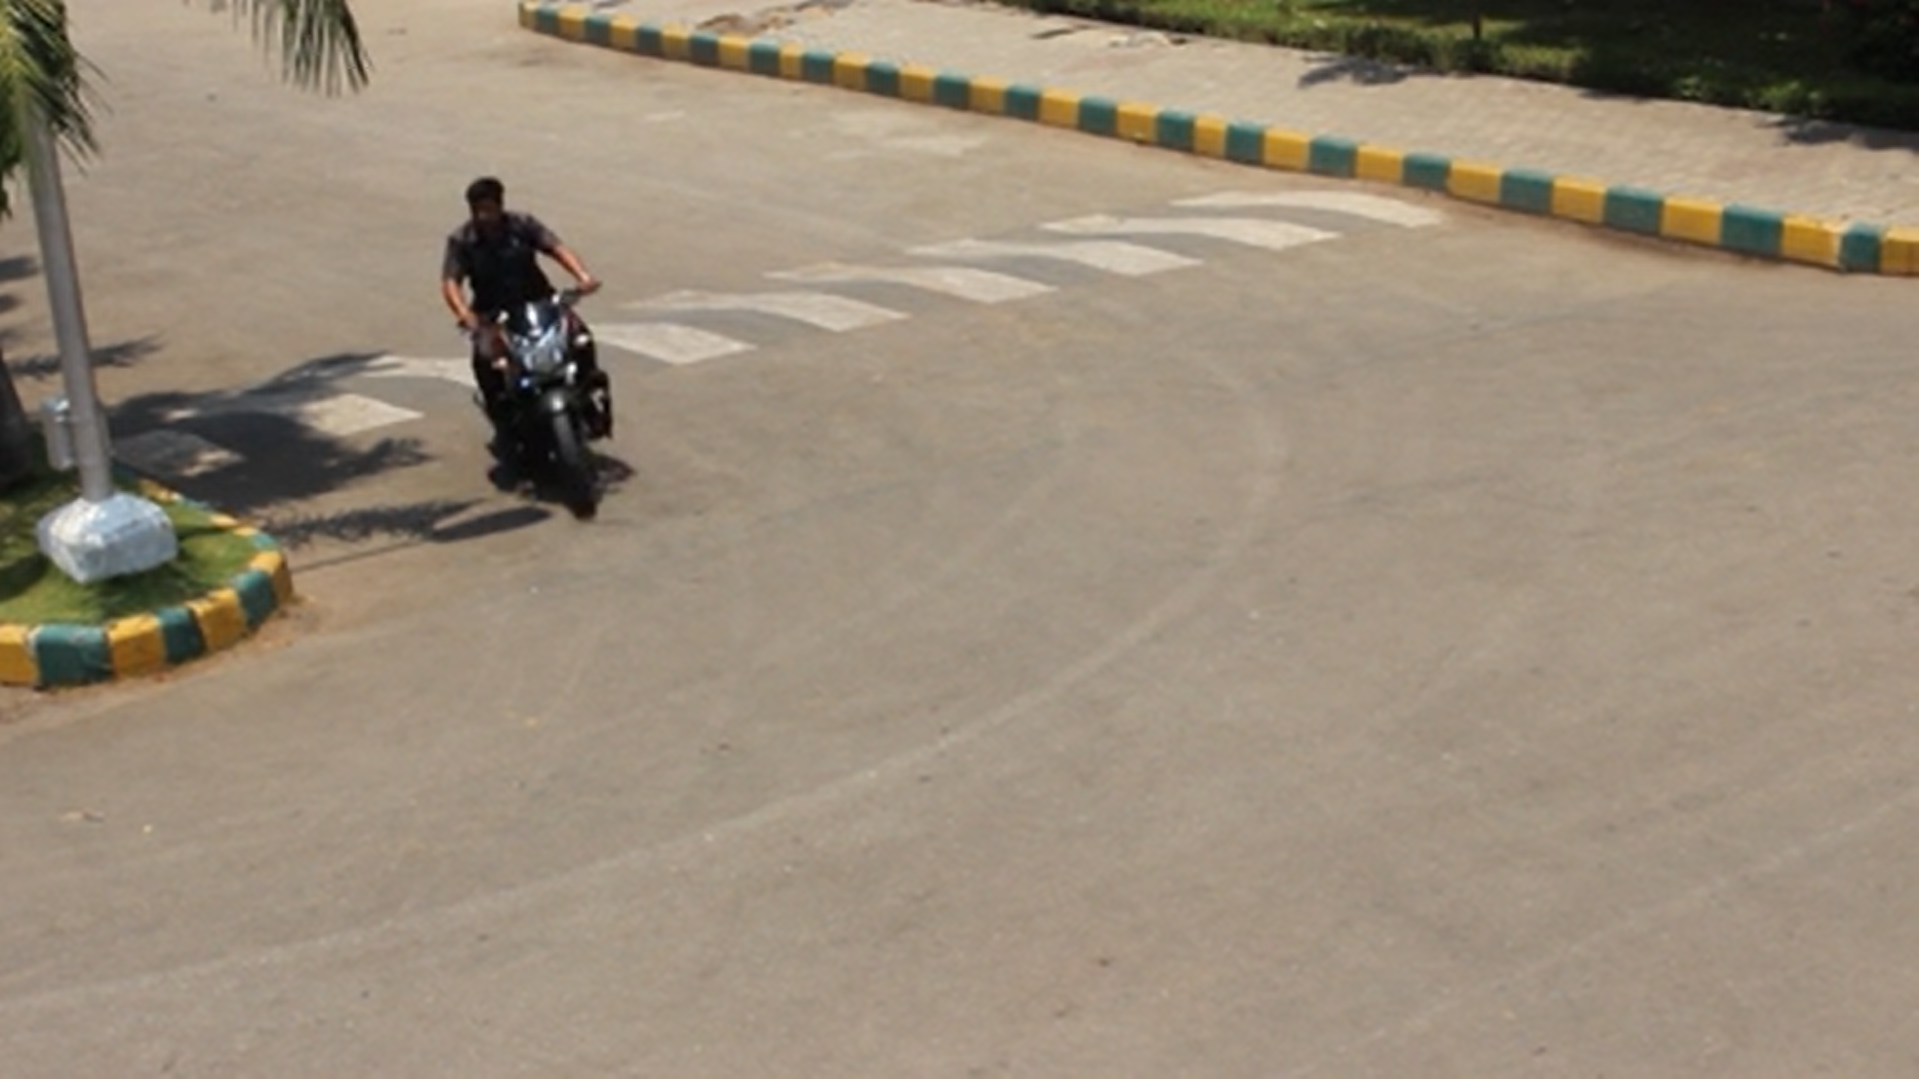
\includegraphics[width=\linewidth]{sample-input-1.png}
    \endminipage\hfill
    \minipage{0.16\textwidth}
        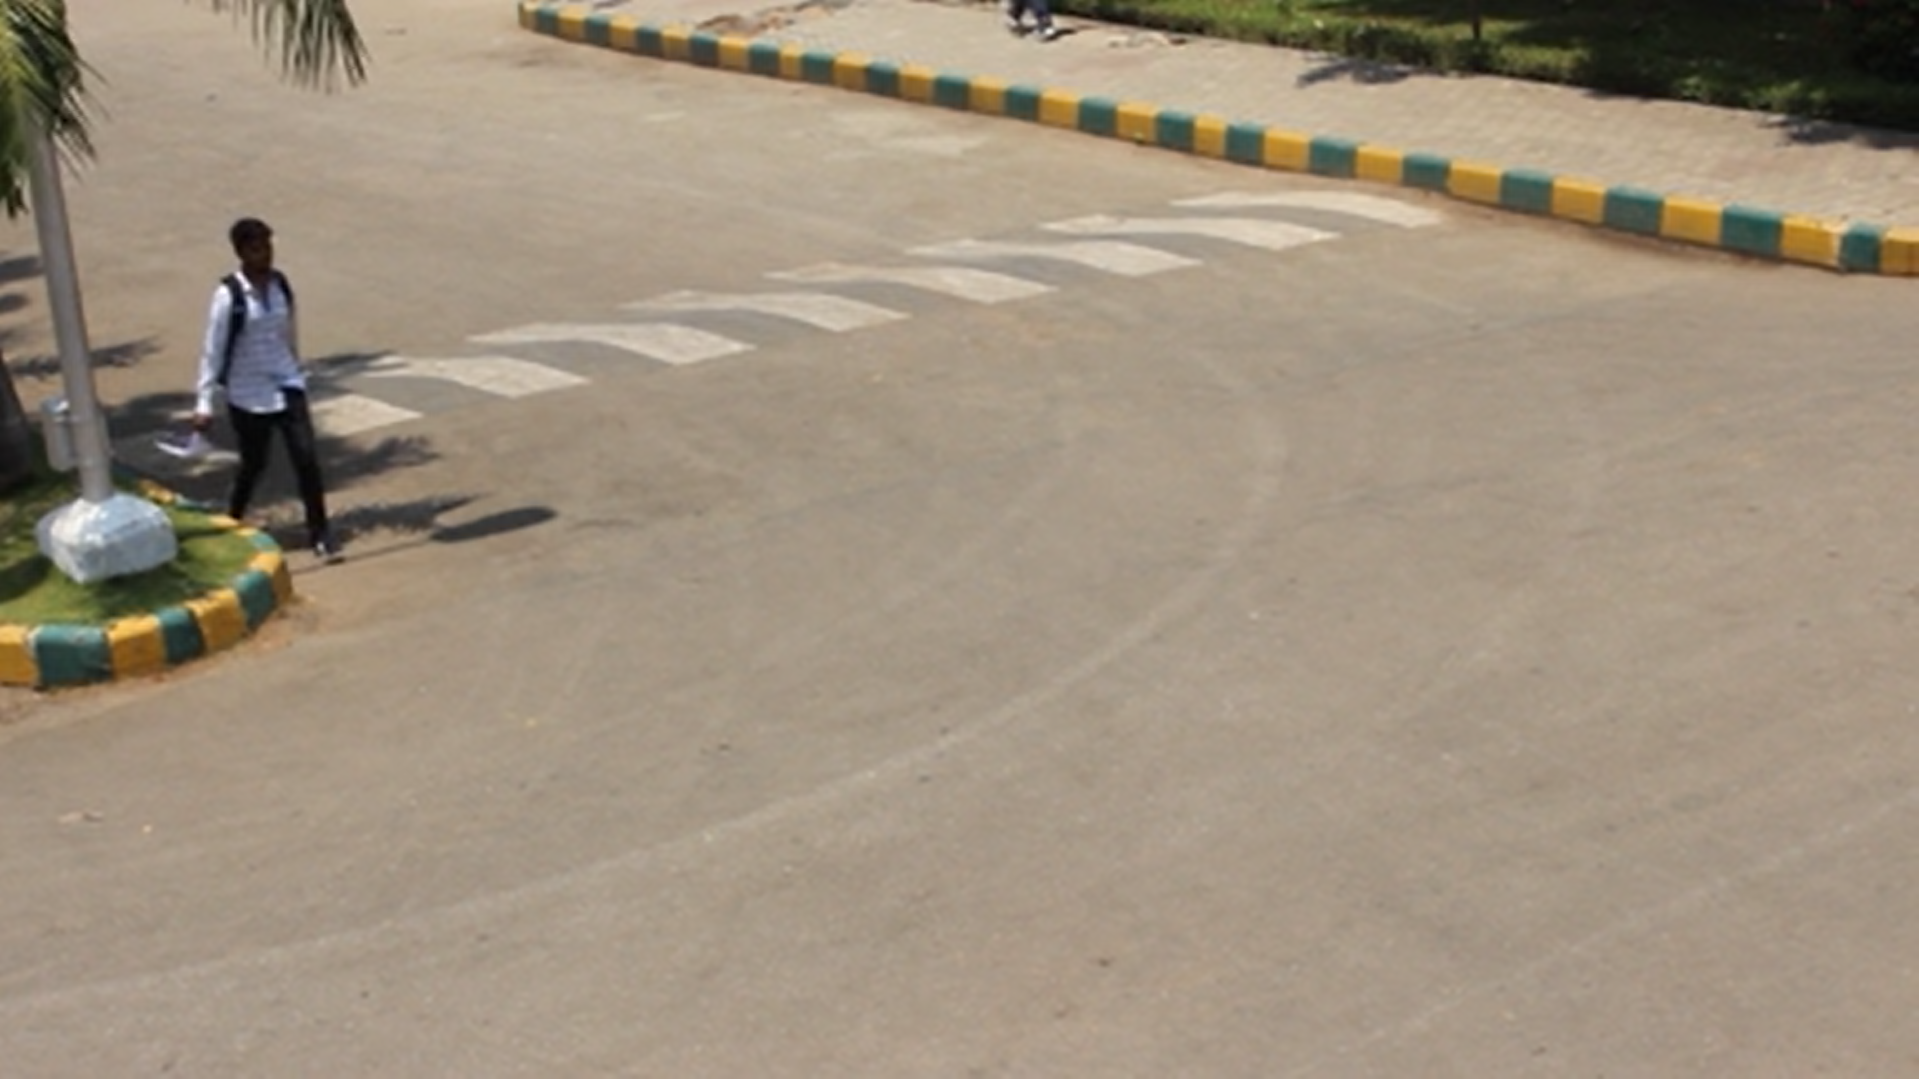
\includegraphics[width=\linewidth]{sample-input-2.png}
    \endminipage\hfill
    \minipage{0.16\textwidth}
        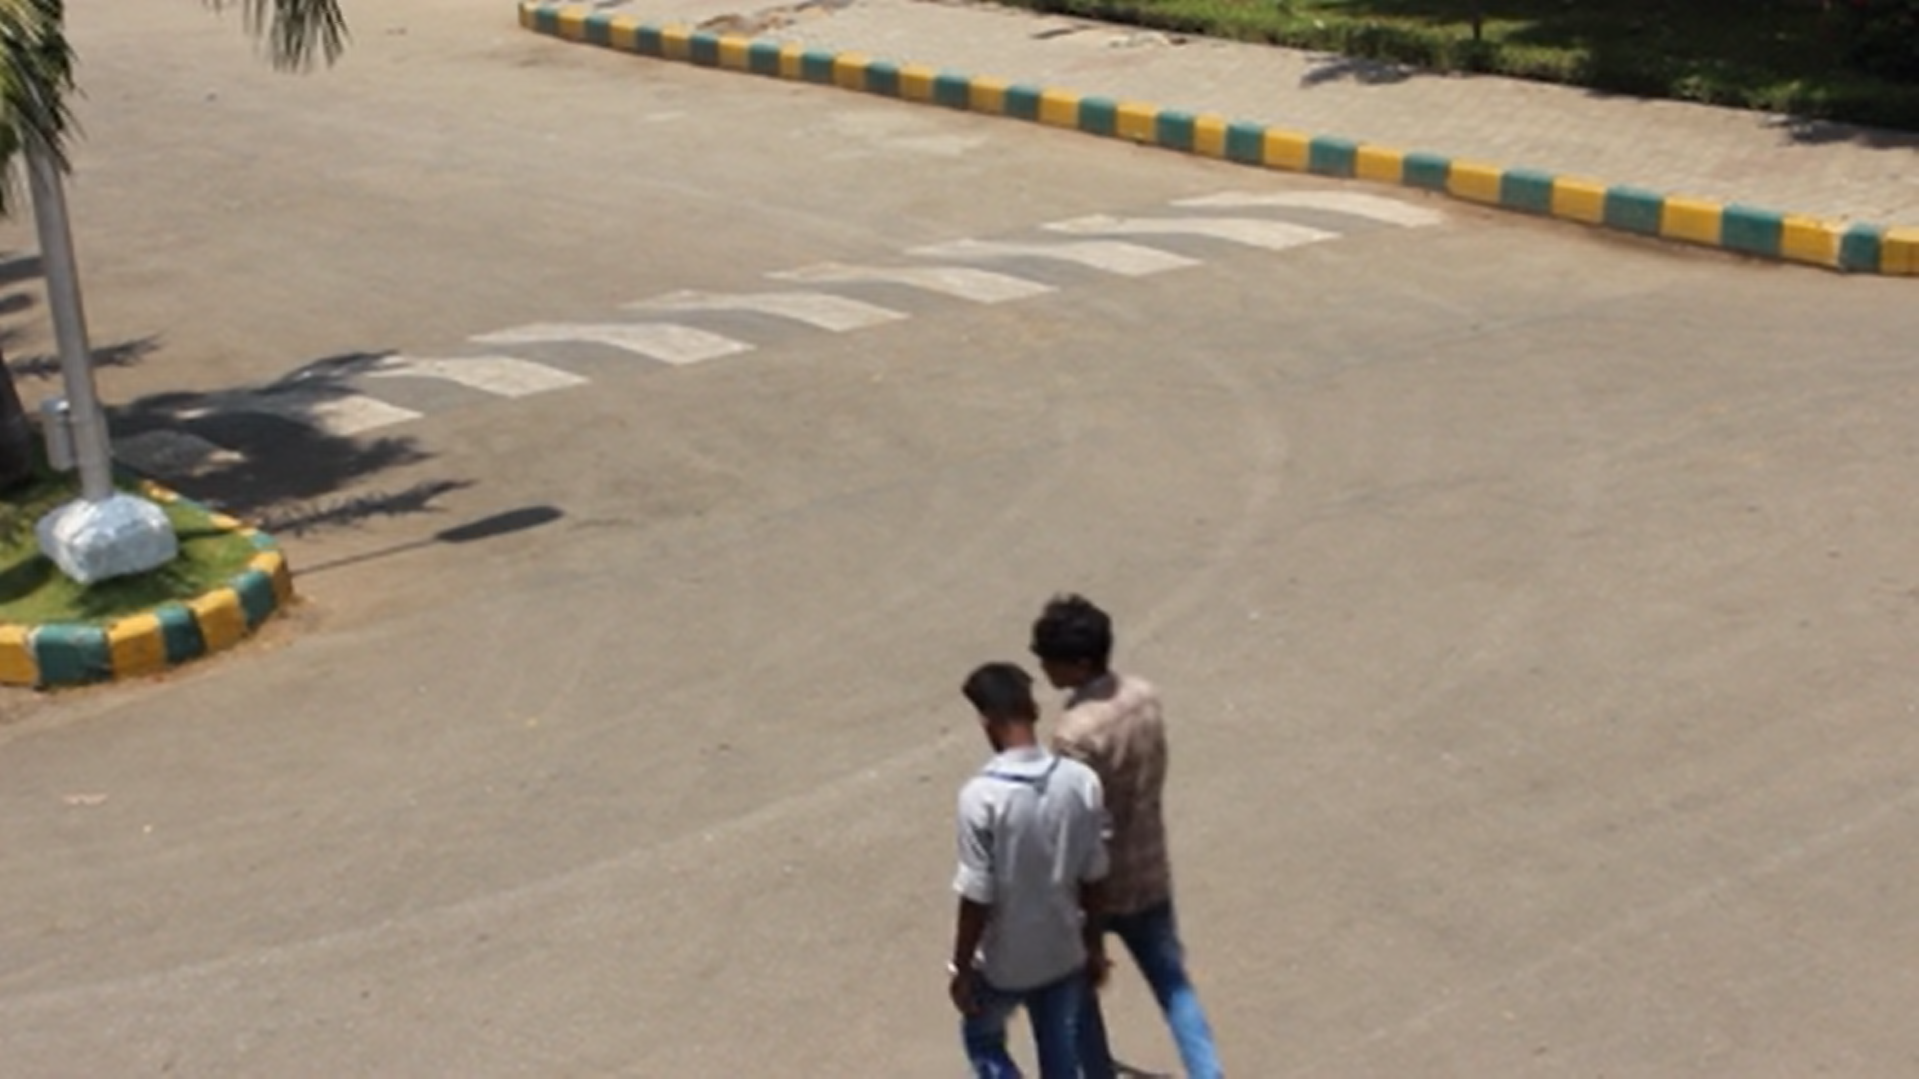
\includegraphics[width=\linewidth]{sample-input-3.png}
    \endminipage
    \caption{Selection of input frames from one of our experimental videos}
    \label{img:sample-input}
\end{figure}

Figure \ref{img:sample-output} shows an output frame generated by our video
summariser. Many people and bikes are seen simultaneously, and the timestamp
shows the time at which the event occurred in the original input video. It is
apparent from this picture that the density of events is dramatically
improved.

\begin{figure}[H]
    \centering
    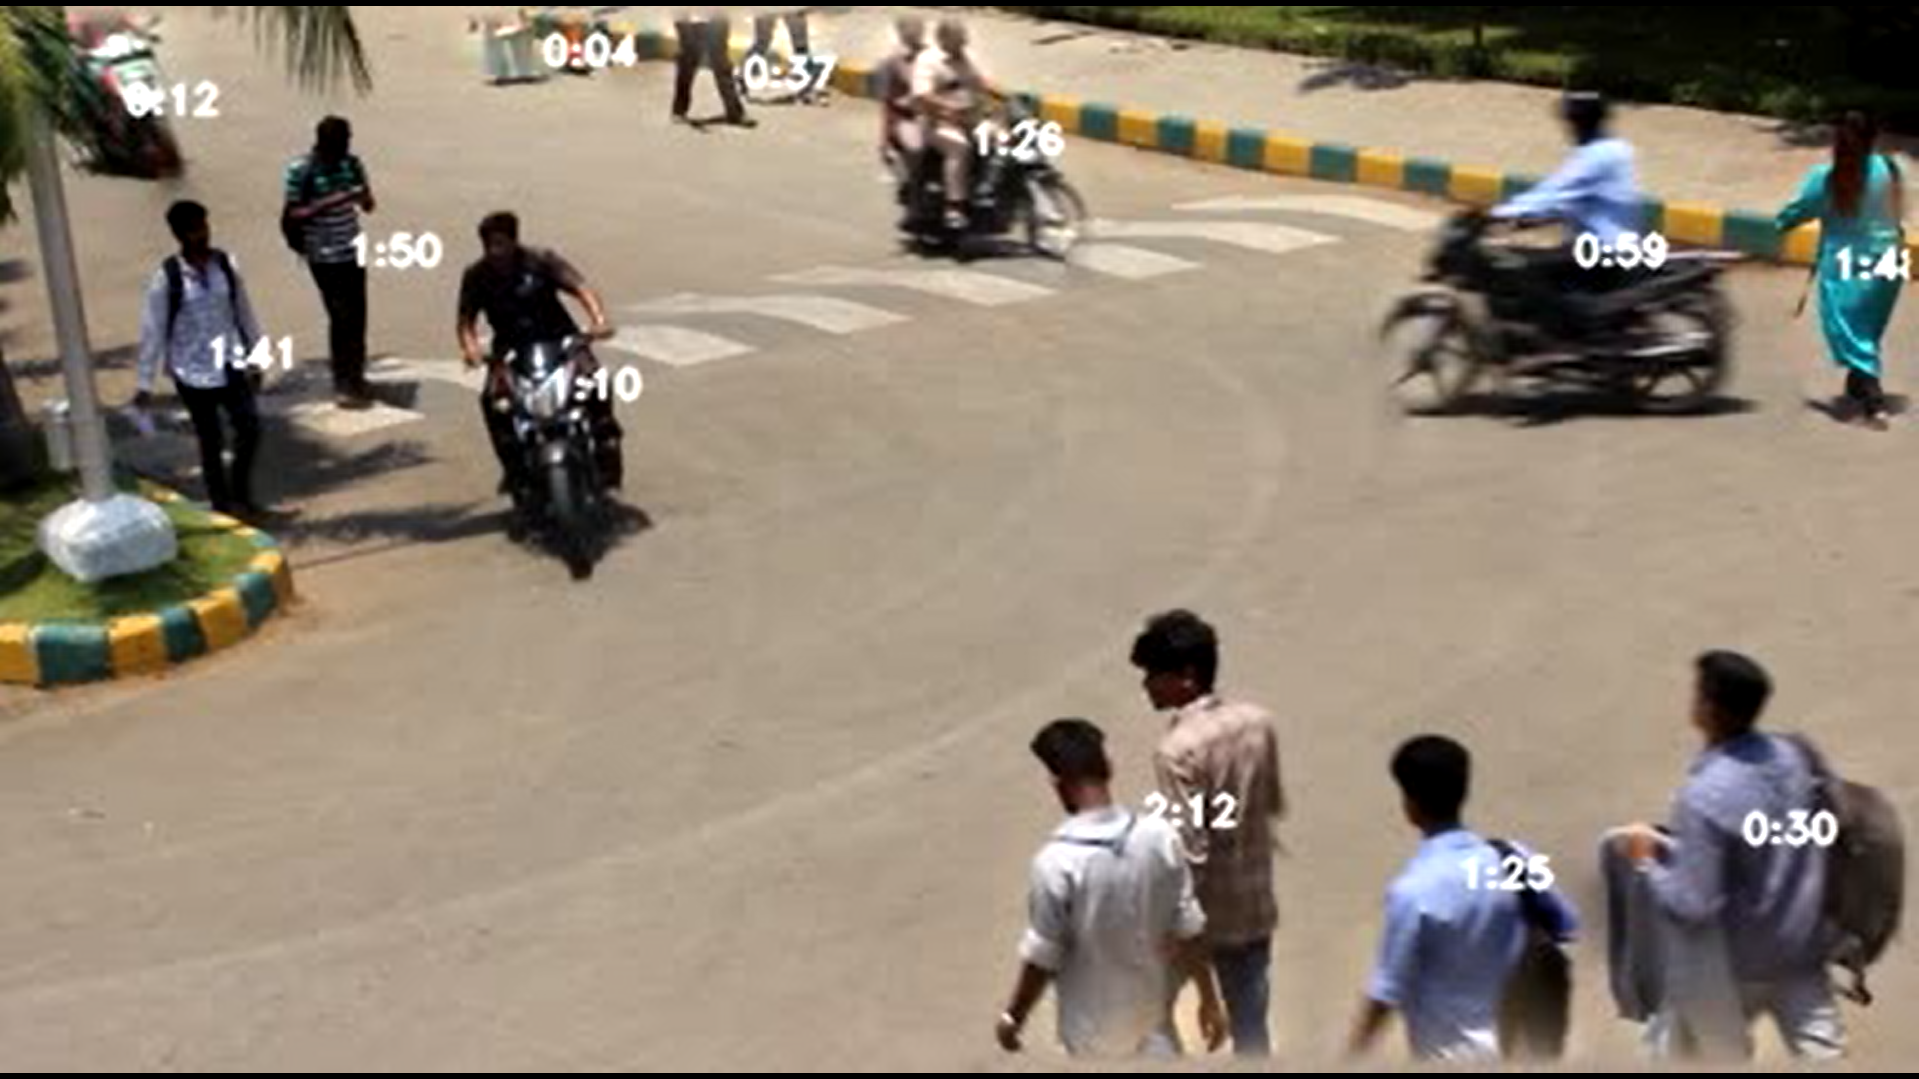
\includegraphics[scale=0.18]{sample-output.png}
    \caption{A frame from the generated summary video}
    \label{img:sample-output}
\end{figure}

\subsection{Objective Evaluation Parameters}

    \begin{itemize}
        \item \textbf{Exhaustiveness of summary}
        The summariser must retain all the events that occurred or the events
        of the specified type in the tag-based summary generation. \\
        Result: All significant events are selected in the events
        \item \textbf{Compression factor}
        Given by Length of original input/Length of summary. The compression
        factor must be as high as possible while keeping the overlap factor to
        a minimum. \\
        Result: There is a compression factor of 4-7x for our sample videos

        \begin{center}
            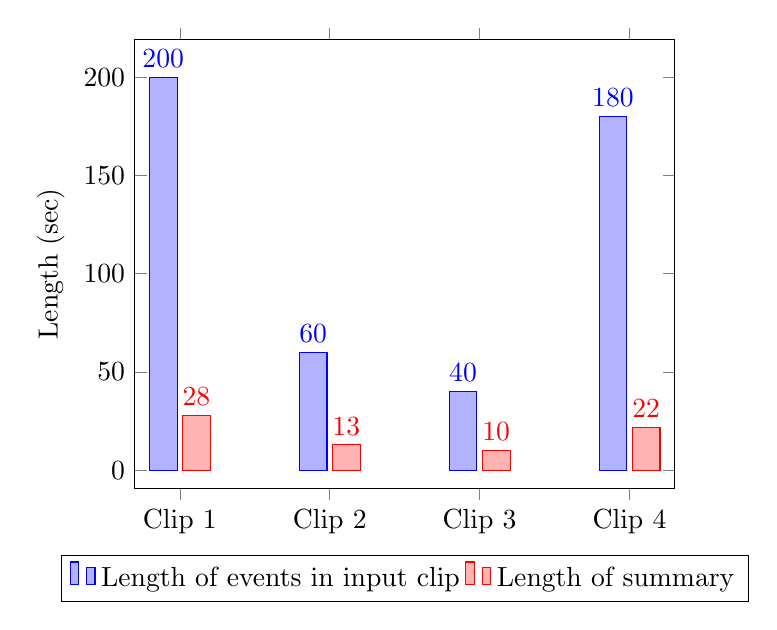
\begin{tikzpicture}
                \begin{axis}[
                    ybar,
                    enlargelimits=0.1,
                    legend style={
                        at={(0.5,-0.15)},
                        anchor=north,legend columns=-1
                    },
                    ylabel={Length (sec)},
                    symbolic x coords={Clip 1, Clip 2, Clip 3, Clip 4},
                    xtick=data,
                    nodes near coords,
                    nodes near coords align={vertical},
                ];
                \addplot coordinates {
                    (Clip 1, 200)
                    (Clip 2, 60)
                    (Clip 3, 40)
                    (Clip 4, 180)
                };
                \addplot coordinates {
                    (Clip 1, 28)
                    (Clip 2, 13)
                    (Clip 3, 10)
                    (Clip 4, 22)
                };
                \legend{Length of events in input clip, Length of summary}

                \end{axis}
            \end{tikzpicture}
        \end{center}


        \item \textbf{Overlap factor}
        A number between 0 and 1 which indicates the amount of overlapping
        (intersection) between the tubes in the summary video. 0 indicates no
        overlap and 1 indicates complete overlap of every clip. \\
        Result: All videos have overlap lower than 0.1
    \end{itemize}

    \subsection{Subjective Evaluation Parameters}

    \begin{itemize}
        \item \textbf{Semantic structure of events}
        Interacting events (that occur in the same time and space) must be
        shown together. \\
        Result: All the interacting events are always shown together
        \item \textbf{Realistic appearance}
        The events must be extracted and be blended into the background
        seamlessly and appear realistic. \\
        Result: Realistic appearance in most cases, with some halo around
        object when at the edges of the frame, or when there is intersection.
    \end{itemize}

\section{Conclusion}
This project aimed to use a novel method to generate video summaries to reduce
the amount of time spent in analyzing CCTV video footage. Our implementation of
summarization by temporal rearrangement of events improves on other methods of
just detecting frames of motion. The tag-based summary selects only the required
type of event, reducing the summary length further.

A proof-of-concept has been presented, and it can be extended to be used in
commercial CCTV systems with further development.

\bibliographystyle{plain} % We choose the "plain" reference style
\bibliography{refs} % Entries are in the "refs.bib" file
\end{document}
